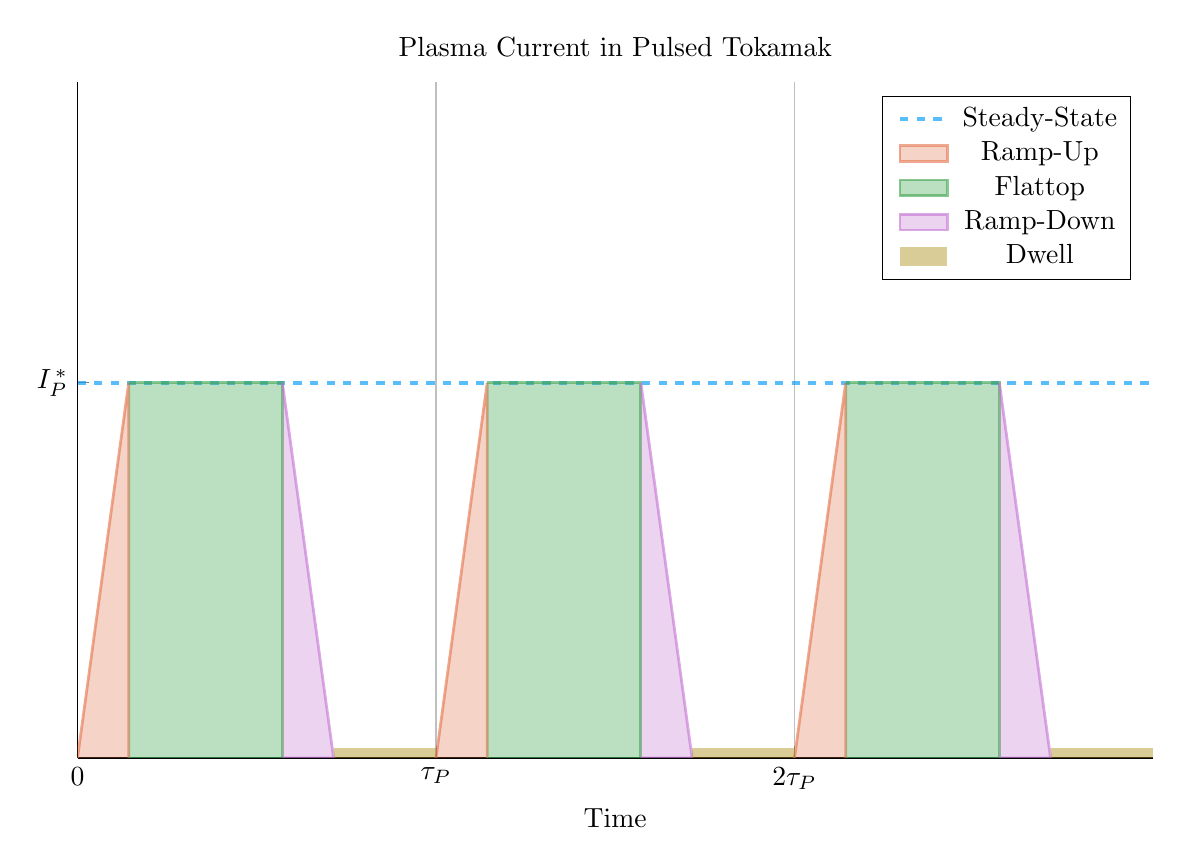
\begin{tikzpicture}[]
\begin{axis}[height = {101.6mm}, ylabel = {}, title = {Plasma Current in Pulsed Tokamak}, xmin = {0.0}, xmax = {21.0}, ymax = {1.8}, xlabel = {Time}, unbounded coords=jump,scaled x ticks = false,xticklabel style={rotate = 0},xmajorgrids = true,xtick = {0,7,14},xticklabels = {0,$\tau_P$,$2 \tau_P$},xtick align = inside,axis lines* = left,scaled y ticks = false,yticklabel style={rotate = 0},ymajorgrids = false,ytick = {1},yticklabels = {$I_P^{\,*}$},ytick align = inside,axis lines* = left,    xshift = 0.0mm,
    yshift = 0.0mm,
    axis background/.style={fill={rgb,1:red,1.00000000;green,1.00000000;blue,1.00000000}}
, ymin = {0.0}, width = {152.4mm}]\addplot+ [color = {rgb,1:red,0.00000000;green,0.60560316;blue,0.97868012},
draw opacity=0.65,
line width=1.5,
dashed,mark = none,
mark size = 2.0,
mark options = {
    color = {rgb,1:red,0.00000000;green,0.00000000;blue,0.00000000}, draw opacity = 0.65,
    fill = {rgb,1:red,0.00000000;green,0.60560316;blue,0.97868012}, fill opacity = 0.65,
    line width = 1,
    rotate = 0,
    solid
}]coordinates {
(0, 1)
(21, 1)
};
\addlegendentry{Steady-State}
\addplot+ [color = {rgb,1:red,0.88887350;green,0.43564919;blue,0.27812294},
draw opacity=0.6,
line width=1,
solid,mark = none,
mark size = 2.0,
mark options = {
    color = {rgb,1:red,0.00000000;green,0.00000000;blue,0.00000000}, draw opacity = 0.6,
    fill = {rgb,1:red,0.88887350;green,0.43564919;blue,0.27812294}, fill opacity = 0.6,
    line width = 1,
    rotate = 0,
    solid
},fill = {rgb,1:red,0.88887350;green,0.43564919;blue,0.27812294}, fill opacity=0.3,area legend]coordinates {
(0.0, 0.0)
(1.0, 1.0)
(1.0, 0.0)
(NaN, NaN)
(7.0, 0.0)
(8.0, 1.0)
(8.0, 0.0)
(NaN, NaN)
(14.0, 0.0)
(15.0, 1.0)
(15.0, 0.0)
};
\addlegendentry{Ramp-Up}
\addplot+ [color = {rgb,1:red,0.24222430;green,0.64327509;blue,0.30444865},
draw opacity=0.6,
line width=1,
solid,mark = none,
mark size = 2.0,
mark options = {
    color = {rgb,1:red,0.00000000;green,0.00000000;blue,0.00000000}, draw opacity = 0.6,
    fill = {rgb,1:red,0.24222430;green,0.64327509;blue,0.30444865}, fill opacity = 0.6,
    line width = 1,
    rotate = 0,
    solid
},fill = {rgb,1:red,0.24222430;green,0.64327509;blue,0.30444865}, fill opacity=0.35,area legend]coordinates {
(1.0, 1.0)
(4.0, 1.0)
(4.0, 0.0)
(1.0, 0.0)
(NaN, NaN)
(8.0, 1.0)
(11.0, 1.0)
(11.0, 0.0)
(8.0, 0.0)
(NaN, NaN)
(15.0, 1.0)
(18.0, 1.0)
(18.0, 0.0)
(15.0, 0.0)
};
\addlegendentry{Flattop}
\addplot+ [color = {rgb,1:red,0.76444018;green,0.44411178;blue,0.82429754},
draw opacity=0.6,
line width=1,
solid,mark = none,
mark size = 2.0,
mark options = {
    color = {rgb,1:red,0.00000000;green,0.00000000;blue,0.00000000}, draw opacity = 0.6,
    fill = {rgb,1:red,0.76444018;green,0.44411178;blue,0.82429754}, fill opacity = 0.6,
    line width = 1,
    rotate = 0,
    solid
},fill = {rgb,1:red,0.76444018;green,0.44411178;blue,0.82429754}, fill opacity=0.3,area legend]coordinates {
(4.0, 1.0)
(5.0, 0.0)
(4.0, 0.0)
(NaN, NaN)
(11.0, 1.0)
(12.0, 0.0)
(11.0, 0.0)
(NaN, NaN)
(18.0, 1.0)
(19.0, 0.0)
(18.0, 0.0)
};
\addlegendentry{Ramp-Down}
\addplot+ [color = {rgb,1:red,0.67554396;green,0.55566233;blue,0.09423434},
draw opacity=0.45,
line width=7,
solid,mark = none,
mark size = 2.0,
mark options = {
    color = {rgb,1:red,0.00000000;green,0.00000000;blue,0.00000000}, draw opacity = 0.45,
    fill = {rgb,1:red,0.67554396;green,0.55566233;blue,0.09423434}, fill opacity = 0.45,
    line width = 1,
    rotate = 0,
    solid
}]coordinates {
(5.0, 0.0)
(7.0, 0.0)
(NaN, NaN)
(12.0, 0.0)
(14.0, 0.0)
(NaN, NaN)
(19.0, 0.0)
(21.0, 0.0)
};
\addlegendentry{Dwell}
\end{axis}

\end{tikzpicture}
